% Beamer Template based on A&M PolSci by Miwa Nakajo. October 24, 2009
% Modified by Kouketu Lyu. Jan. 6th, 2025 without any warnings.
% This templater is used for the persentation in ISEE of KYUSHU UNIVERSITY.

\documentclass[]{beamer} % option [handout]or[trans]
\usepackage{hyperref}
% if don't disable the commands \translate, there will be a warning.
% I can't solve this problem, so did like below. If you can, try it!
\pdfstringdefDisableCommands{%
    \def\translate#1{#1}
}  
\usepackage{multirow}
\usepackage{graphicx} % for A&M Logo
\usepackage[round]{natbib}
\usepackage{float}
\usepackage{animate}
\usepackage[utf8]{inputenc}
\usepackage[T1]{fontenc} 
\usepackage{colortbl}
\usepackage{amssymb}
\usepackage{siunitx}
\usepackage{tikz}
\usepackage{makecell}
\usepackage{booktabs}
\usepackage{tabularx}
\usepackage{array}
\usepackage{cite}
\usepackage{color}
\usepackage{dcolumn}
\usepackage{listings}
\usepackage{subcaption}


\newcommand{\backupbegin}{
    \newcounter{framenumberappendix}
    \setcounter{framenumberappendix}{\value{framenumber}}
}

\newcommand{\backupend}{
    \addtocounter{framenumberappendix}{-\value{framenumber}}
    \addtocounter{framenumber}{\value{framenumberappendix}} 
}
% \usepackage[paperwidth=12cm,paperheight=5cm]{geometry}
\title[short\_title]{Your Title}

% \subtitle{}
\author{First FAMILY}
    %\author{Your Name\inst{1} \and Coauthor's Name\inst{2}}
\institute{INSTITUTE}
    %\institute{\inst{1}Texas A\&M University \and \inst{2}Other University}
\date{\small{Jul. 5th, 2024}}
    %\date{POLS601, \today}
\titlegraphic{\includegraphics[width=0.3\paperwidth]{logo/kyushu\_isee\_logo.pdf}}

\useinnertheme{default}
    % or {rectangles}, {circles}, {rounded}
\useoutertheme{default}
    % other options do not work with this template. You might not need this line.

% font
\usefonttheme{default}

% color
\definecolor{light}{RGB}{132,5,61} % A&M's primary color
\definecolor{332C2C}{RGB}{51,44,44} % A&M's primary support color, dark gray
\definecolor{dark}{RGB}{87,30,56} % A&M's secondary colors
\usecolortheme[named=light]{structure}
\setbeamercolor{frametitle}{fg=light,bg=white}
\setbeamercolor{primary}{fg=white,bg=light}
\setbeamercolor{secondary}{fg=white,bg=dark}

% headline
\setbeamertemplate{headline}{
\hbox{%
    \begin{beamercolorbox}[wd=0.5\paperwidth,ht=2.25ex,dp=1ex,left]{primary}
        \hspace*{2ex}\insertsectionhead % Section Title in Left
    \end{beamercolorbox}%
    \begin{beamercolorbox}[wd=0.5\paperwidth,ht=2.25ex,dp=1ex,left]{secondary}
        \hspace*{2ex}\insertsubsectionhead % Subsection Title in Right
    \end{beamercolorbox}}
\vskip0pt }

% footline
\setbeamertemplate{footline}{
\hbox{%
    \begin{beamercolorbox}[wd=.50\paperwidth,ht=2.25ex,dp=1ex,left]{primary}
        \hspace*{2ex}{} % Something in Left
    \end{beamercolorbox}%
%    \begin{beamercolorbox}[wd=.02\paperwidth,ht=2.25ex,dp=1ex,center]{primary}
%       \includegraphics[height=2.25ex,dp=2.25ex]{aTm08-box} % aTm Logo in the Middle
%    \end{beamercolorbox}%
    \begin{beamercolorbox}[wd=.50\paperwidth,ht=2.25ex,dp=1ex,right]{primary}
        \insertframenumber{} / \inserttotalframenumber \hspace*{3ex} % Page numbers in Right
    \end{beamercolorbox}}
\vskip0pt }

\let\Tiny=\tiny

\AtBeginSection[]
{
  \begin{frame}
    \frametitle{}
    \tableofcontents[currentsection,subsectionstyle=show/show/shaded]
  \end{frame}
}




% Slides Start
\begin{document}

% Title Page
\frame{\titlepage}
\section{Background \& Related Works}


\frame
{\frametitle{German to Upper Sorbian NMT}

\begin{figure}
  \centering
  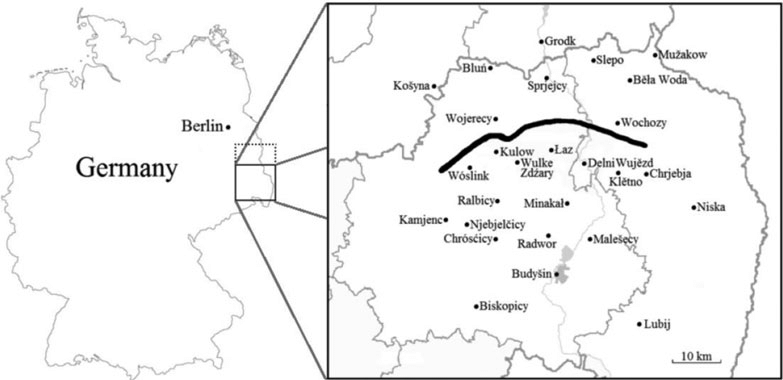
\includegraphics[width=0.8\textwidth, keepaspectratio]{figure/Location-of-the-Upper-Sorbian.png}
  \caption{Upper Sorbian is spoken south of the solid black line. Image taken from \citep{howson2017upper}. }
\end{figure}

}

\frame
{\frametitle{Related works: Back Translation}

Back-translation is a popular data augmentation technique to \textcolor<1>{red}{expand parallel corpora} to enhance model performance.  

\begin{itemize}
    \item<2-4> A proposed method utilizes a monolingual corpus on \textcolor<2>{red}{the target side} for back-translation \citep{sennrich-etal-2016-improving}.  
    \item<3-4> \citet{fadaee-monz-2018-back} investigated various aspects of back-translation and proposed several \textcolor<3>{red}{sampling strategy variations}. 
    \item<4> Additionally, \textcolor<4>{red}{iterative back-translation} to expand low-resource corpora was explored by \citep{hoang-etal-2018-iterative}. 
\end{itemize}
}


\section{Data}

\frame
{\frametitle{Data}
\begin{table}
	\begin{center}
    \resizebox{\columnwidth}{!}{
		\begin{tabular}{llccr}
			\toprule
			    \multirow{2}*{Corpus} & \multirow{2}*{Language} & \multirow{2}*{\# sentences} & \multicolumn{2}{c}{Sentence length}  \\
				\cline{4-5}
				~                     &            ~          &                ~             & in words             & in characters \\
			\midrule
				\multirow{2}*{Bilingual} &  German (de)       &  \multirow{2}*{60,000 $\times$ 2}   & 12.1 ± 6.9           & 83.4 ± 51.7 \\
						~			  &  Upper Sorbian (hsb)  &                ~             & 10.7 ± 6.3           & 71.6 ± 45.4\\
			\midrule
				Monolingual  		&       German (de)		  &            1,879,765         &	15.4 ± 9.2			&	108.5 ± 64.8 \\
			\bottomrule
		\end{tabular}
    }	
		\caption{Statistics of the corpora.}
		\label{table:Statistics of the Corpora}
	\end{center}
\end{table}
We use the German-Upper Sorbian (de-hsb) parallel corpus from WMT20\footnote{https://www.statmt.org/wmt20/unsup\_and\_very\_low\_res/} as the original bilingual corpus, while the German corpus from WMT14\footnote{\url{https://www.statmt.org/wmt14/training-monolingual-news-crawl/}} is chose as the original monolingual corpus.
}

\frame
{\frametitle{Thank you}
  \centerline{Thanks for your attention!}
}

\backupbegin

% Appendix
\section{}
\frame
{\frametitle{Related works: Back Translation}
% nothing
% \only<1>{
% \begin{figure}
%   \centering
%   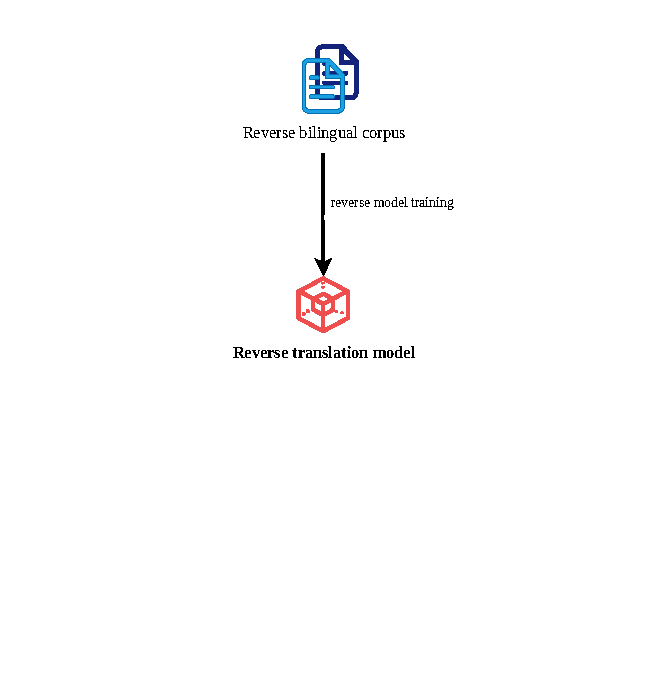
\includegraphics[width=0.6\textwidth, keepaspectratio]{figure/BT/backtranslation_1.pdf}
%   \caption{Back Translation procedure. \citep{sennrich-etal-2016-improving}}
% \end{figure} 
% }
% \only<2>{
% \begin{figure}
%   \centering
%   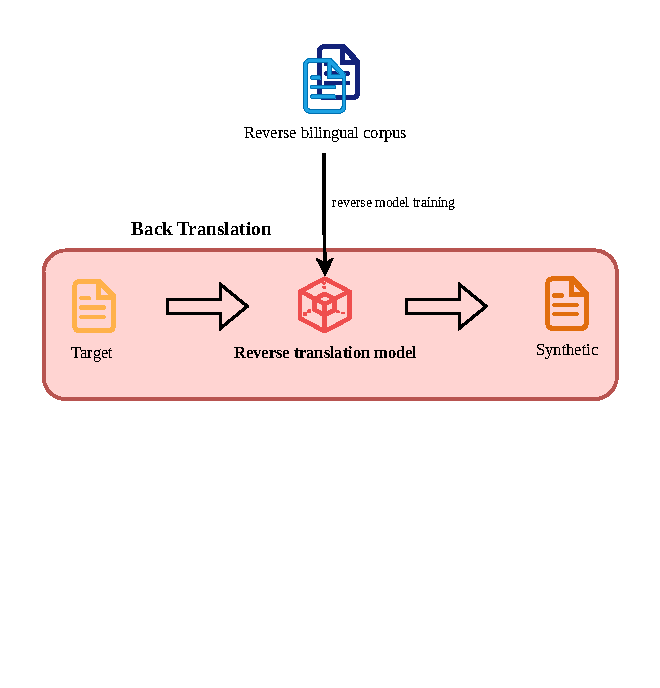
\includegraphics[width=0.6\textwidth, keepaspectratio]{figure/BT/backtranslation_2.pdf}
%   \caption{Back Translation procedure. \citep{sennrich-etal-2016-improving}}
% \end{figure} 
% }
% \only<3>{
% \begin{figure}
%   \centering
%   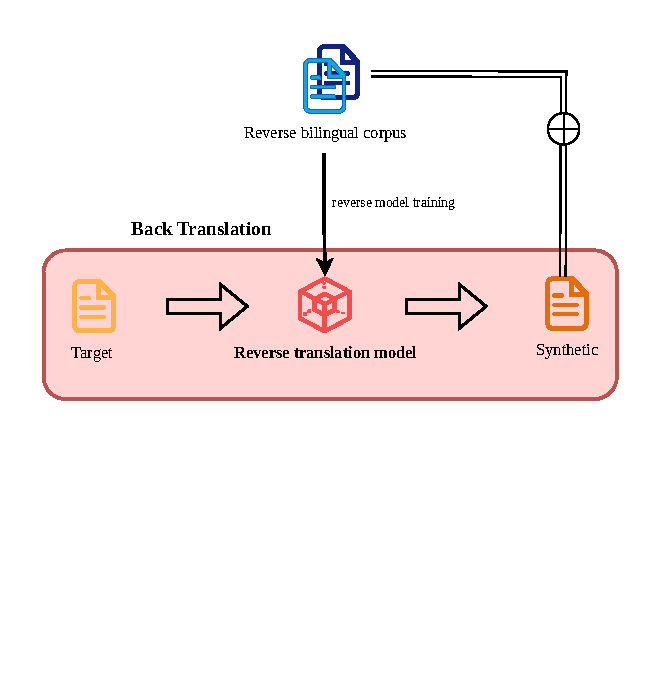
\includegraphics[width=0.6\textwidth, keepaspectratio]{figure/BT/backtranslation_3.pdf}
%   \caption{Back Translation procedure. \citep{sennrich-etal-2016-improving}}
% \end{figure} 
% }
% \only<4>{
% \begin{figure}
%   \centering
%   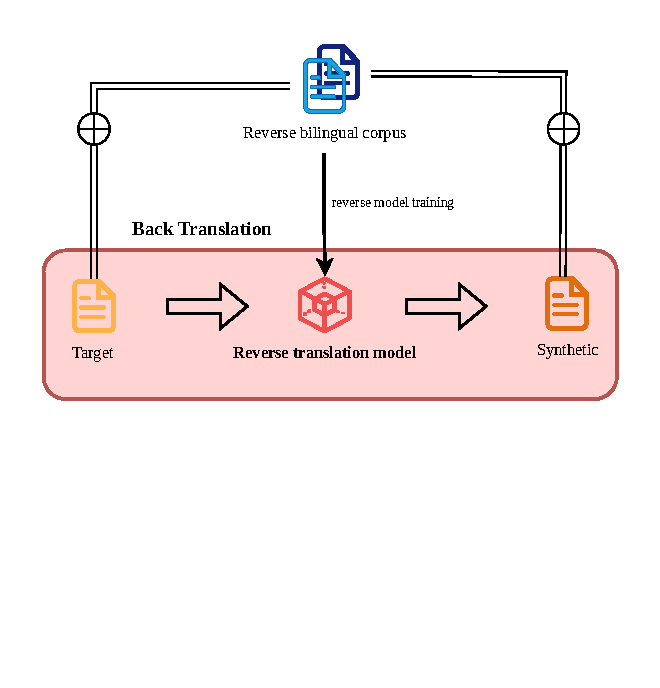
\includegraphics[width=0.6\textwidth, keepaspectratio]{figure/BT/backtranslation_4.pdf}
%   \caption{Back Translation procedure. \citep{sennrich-etal-2016-improving}}
% \end{figure} 
% }

\begin{figure}
  \centering
  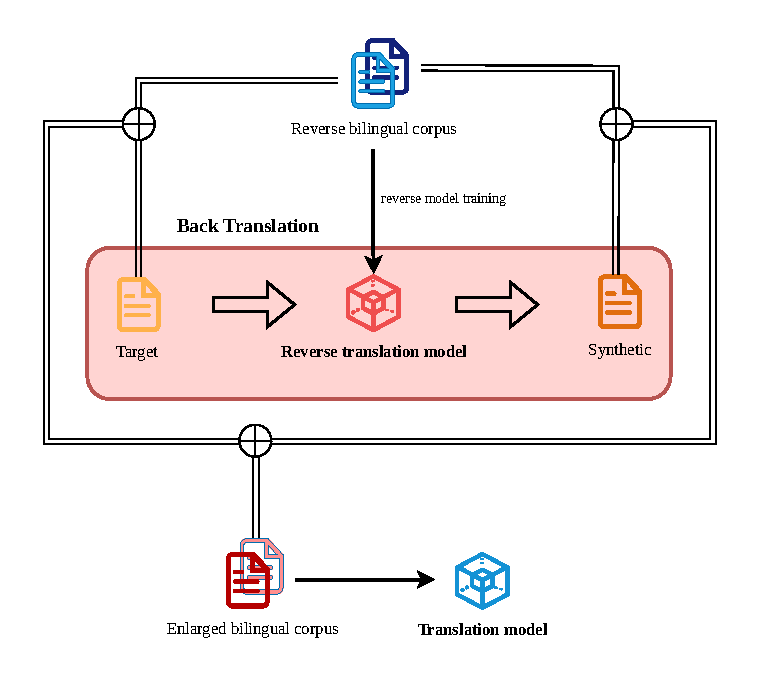
\includegraphics[width=0.7\textwidth, keepaspectratio]{figure/BT/backtranslation.pdf}
  \caption{\citep{sennrich-etal-2016-improving}}
\end{figure} 
 } 

% References
\begin{frame}[allowframebreaks]{References}

\renewcommand{\bibname}{References}
\small
\bibliographystyle{plainnat}
\bibliography{references}

\end{frame}


\backupend
\end{document}

